
Com o intuito de planejar a Verificação e Validação da Interface Gráfica que compõe o sistema Enturma, primeiramente precisamos compreender as funcionalidades principais do sistema, seu objetivo principal, seus objetivos secundários e os pontos mais críticos do sistema.

O sistema Enturma possui como objetivo, informar a população brasileira sobre o desempenho das turmas escolares no país, facilitando o conhecimento a cerca da distribuição de ensino por todo o país, apresentando com clareza as diferenças entre cada estado e seus tipos escolares (público, privado, estadual, municipal). 

Obter a informação a cerca de uma determinada turma é o principal objetivo do sistema, já que o usuário poderá saber a evolução de sua turma, podendo compará-la com outras turmas, de outros estados por exemplo. O \textit{framework do problema} pode ser observado na tabela \ref{tab:problema}.


\begin{table}[H]
	\centering
	\begin{tabular}{|l|l|}
		\hline
		\textbf{O problema de}                    & \begin{tabular}[c]{@{}l@{}}Falta de conhecimento a cerca do desempenho\\ das turmas escolares brasileiras.\end{tabular}                                                                                                                                                                         \\ \hline
		\textbf{Afeta}                            & Todos os brasileiros.                                                                                                                                                                                                                                                                           \\ \hline
		\textbf{Cujo impacto é}                   & \begin{tabular}[c]{@{}l@{}}O decaimento do rendimento dos alunos fica a margem \\ do conhecimento da população brasileira, estando essa \\ sem ter como acompanhar quando é que a educação \\ começa a oscilar para poder exigir investimento de \\ recursos por parte do governo.\end{tabular} \\ \hline
		\textbf{Benefícios de uma solução seriam} & \begin{tabular}[c]{@{}l@{}}Exigência por parte da população para a elaboração de \\ leis e medidas que focariam melhorias na educação em \\ fases críticas do ensino, as quais se apresentam \\ defasadas nos resultados das provas avaliativas.\end{tabular}                                   \\ \hline
	\end{tabular}
	\caption{Framework de Problema}
	\label{tab:problema}
\end{table}

\subsection{Recursos do produto} % (fold)
\label{sub:recursos_do_produto}


Os usuários finais do sistema EnTurma possuem como maior necessidade a de visualizar o desempenho de uma determinada turma do sistema educacional brasileiro. A tabela \ref{tab:recursos} apresenta todos os recursos do sistema e suas características.

\begin{table}[H]
	\centering
	\begin{tabular}{|l|l|}
		\hline
		\textbf{Necessidade}      & \textbf{Características}                                                                                                                                                                                                                                                                                                   \\ \hline
		Gerar relatório da turma  & \begin{tabular}[c]{@{}l@{}}Os gráficos podem ser gerados a partir dos indicadores \\ e período escolhidos. Os indicadores podem ser: média\\  dos alunos, média de horas/aula, taxa de rendimento, \\ e outros. O período escolhido pode variar entre 2006 a \\ 2014 dependendo da disponibilidade dos dados.\end{tabular} \\ \hline
		Comparar turmas           & \begin{tabular}[c]{@{}l@{}}Comparação de duas turmas em um mesmo indicador. \\ Exemplo: comparar a turma da primeira série do ano \\ de 2007 com a de 2008 em relação à média escolar.\end{tabular}                                                                                                                        \\ \hline
		Gerar ranking             & \begin{tabular}[c]{@{}l@{}}O sistema deve gerar ranking dos melhores estados em \\ um determinado indicador.\end{tabular}                                                                                                                                                                                                  \\ \hline
		Contactar desenvolvedores & \begin{tabular}[c]{@{}l@{}}O sistema disponibiliza uma seção que permite que o \\ usuário entre em contato com os desenvolvedores a fim \\ de sanar dúvidas, fazer críticas ou sugestões sobre o sistema.\end{tabular}                                                                                                     \\ \hline
	\end{tabular}
	\caption{Recursos do Sistema}
	\label{tab:recursos}
\end{table}

	O relacionamento destes recursos com os Atores do sistema pode ser observado na Modelagem de Casos de Uso do Sistema Enturma, que está disposta na figura \ref{img:modelagem}.

	\begin{figure}[H]
		\centering
		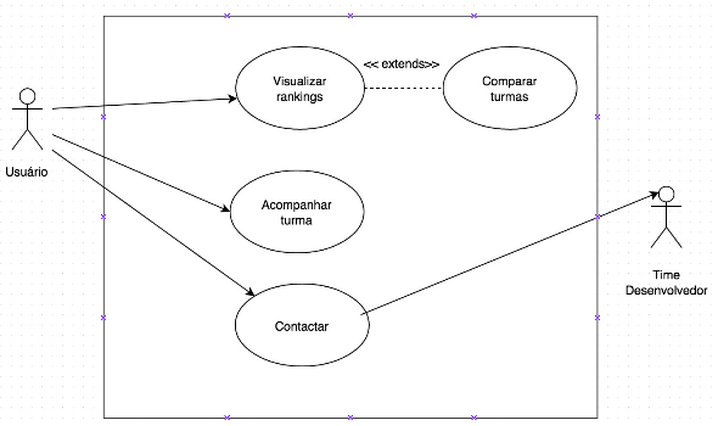
\includegraphics[width=0.7\textwidth]{imagens/modelagem}
		\caption{Modelagem de Casos de Uso}
		\label{img:modelagem}
	\end{figure}




\subsection{Técnicas de Questionario}
	Técnicas de questionario são aplicadas em testes de usabilidade em que há participação do usuario com o objetivo de perguntar ao usuario sobre a interface do software com o objetivo de descobrir se o software esta suprindo as necessidades do usuario.

	Na maioria das vezes um modelo de questionário apóia-se nas experiências e
	heurísticas de seus elaboradores. Quando é utilizado em pesquisas reais ou simuladas, o
	modelo depara-se com circunstâncias e necessidades não previstas inicialmente, o que
	determinará os refinamentos e ajustes, que, aplicados sucessivamente, permitirão a
	evolução das questões (NIELSEN; MACK, 1994). 
	
	As técnicas são úteis para se obter detalhes que do ponto de vista nós desenvolvedores não estamos acostumados, e são utilizadas para obter informações relativas as necessidades dos usuarios e revelar possiveis problemas que nós desenvolvedores normalmente nao veriamos.
	
	Serão realizados questionarios afim de se obter dados quantativos, o questionario também tem como vantagem atingir um numero maior de usuarios o que facilita ainda mais a coleta de dados relevantes a respeito do desing do software.
	
	


\subsection{Planejamento da avaliação de usabilidade e questionario de satisfação dos usuários}
	A avaliação da usabilidade será realizada com a utilização do software enturma, facilitando o registro de problemas encontrados durante a utilização do sistema pelos usuários da aplicação.
	A proposta do questionario a ser aplicado aos usuários após a realização da avaliação de usabilidade com base no WAMMI (Website Analysis and MeasurMent Inventory) e no QUIS(Questionnaire for User Interactional Satisfaction).


	O QUIS é uma ferramenta que foi desenvolvida por pesquisadores do Human Computer Interaction Laboratory (HCIL) da University of Maryland, para medir a satisfação do usuario focando em objetivos especificos da interface humano-computador.
	As questões são apresentadas na forma de afirmações
utilizando as escalas de diferencial semântico, que
baseiam-se em explorar uma faixa de atitudes bipolares
representada por um par de adjetivos. As questões são
respondidas em uma escala que varia de O a 9, onde o zero
representa um adjetivo negativo e os demais representam
adjetivos positivos. Por ser um questionário geral utilizado
para uma ampla variedade de produtos, também inclui a
opção N/A (não-aplicável). A Figura 1 mostra um exemplo
de uma questão com escalas de satisfação específica. ( Filardi; Traina, 2008)

\begin{table}
{Exemplo de uma questão de QUIS utilizando escala de diferencial semantico}
\centering
\begin{tabular}{|c|c|c|c|c|c|c|c|c|c|c|c|c|c|c|} 

\hline
   QUIS &  & 1 & 2 & 3 & 4 & 5 & 6 & 7 & 8 & 9 & N/A &  \\
\hline
Mensagens que aparecem na tela & Confusa &  &  &  &  &  &  &  &  &  &  & clara \\ 

\hline
\end{tabular}
\caption {Fonte:Filardi; Traina, 2008}

\end{table}

	O WAMMI é um serviço exclusivo para avaliação de
Websites on-Iine, com o propósito de ajudar os proprietários
do site a cumprir suas metas corporativas através da
medição e monitoramento das reações do usuário sobre
suafacilidade de uso. Através de um botão colocado no site,
é disponibilizado um questionário com a estrutura de um
formulário para ser preenchido. Os dados do questionário
são armazenados e analisados a partir de uma base de dados
padronizada com escores normalizados. São utilizados para
avaliar os seguintes aspectos: atratividade, controle,
eficiência, utilidade, aprendizagem e usabilidade global.
	
	O WAMMI tem como objetivo: 

• medir a satisfação do usuário sobre o site baseado na
reação do usuário;

• gerar dados objetivos de gestão em um formato fácil de
entender;

• prover uma base para mudanças do Website e melhorias
de design;

• comparar seu site em relação aos demais em termos de
satisfação do usuário; 

• acompanhar o desempenho do Website para verificar se
as metas estão sendo cumpridas.

Fonte:Filardi; Traina, 2008
% subsection recursos_do_produto (end)